% ============================================================================
%  TrustFin-SLM — Phase-4 Conference-Paper Draft
%  Execution-Verified Generation with Agreement-Calibrated Abstention
%  for Trustworthy Small Language Models in Finance
%
%  DRAFT (guide stage 15,17,19,20). Compiles with plain pdflatex (article class).
%  For submission, switch to the venue's class (IEEEtran / ACL acl-latex) —
%  content is 1:1, only the header changes. All claims sourced from
%  docs/exp_4(a).md, docs/exp_4(b).md and the phase-4 freeze manifests.
% ============================================================================
\documentclass[conference]{IEEEtran}
\usepackage[utf8]{inputenc}
\usepackage[T1]{fontenc}
\usepackage{lmodern}
\usepackage{microtype}
\usepackage{amsmath,amssymb}
\usepackage{booktabs}
\usepackage{graphicx}
\usepackage[table]{xcolor}
\usepackage{enumitem}
\usepackage{algorithm}
\usepackage{algpseudocode}
\usepackage{tikz}
\usetikzlibrary{arrows.meta,positioning,fit}
\usepackage{url}
\usepackage[numbers,square,sort&compress]{natbib}
\usepackage[colorlinks=true,linkcolor=blue,urlcolor=blue,citecolor=blue]{hyperref}
\graphicspath{{../artifacts/phase4/plots/}{trust_fin_extra_phase/artifacts/phase4/plots/}{../../paper/figures/}{../../artifacts/phase3/plots/}}

\newcommand{\ourmethod}{EVG-CAS}
\newcommand{\RR}{\mathcal{R}}
\newcommand{\CC}{\mathcal{C}}
\newcommand{\p}{\hat p}
\title{\textbf{FinTrust: Trustworthy Small Language Models for Financial Tasks}}
\author{\IEEEauthorblockN{Heet Mehta, Krish Patel, and Aryan Patel}
\IEEEauthorblockA{\href{mailto:heetmehta.work@gmail.com}{heetmehta.work@gmail.com}\\
\href{mailto:krishpatel19.tech@gmail.com}{krishpatel19.tech@gmail.com}\\
\href{mailto:aryanpatel26.ce@gmail.com}{aryanpatel26.ce@gmail.com}}}
\date{}

\begin{document}
\maketitle

\begin{abstract}
Small language models can reduce the cost of financial analysis, but accuracy alone does
not reveal whether a numerical answer should be trusted. We present EVG-CAS, an
execution-verified generation and agreement-calibrated abstention procedure, evaluated on
a frozen QLoRA-adapted 1.7B financial model. The model samples eight candidate programs,
executes valid candidates with the official FinQA evaluator, and uses agreement among the
executed answers as a selective-risk feature. All model and threshold choices are frozen
on validation data before protected evaluation. On the protected FinQA test, EVG-CAS does
not improve accuracy: execution-verified selection obtains 65.56\%, compared with 65.74\%
for greedy decoding (McNemar exact $p=0.871$). It does, however, provide a strong ranking
signal for abstention: agreement-bin accuracy increases from 2.9\% to 79.2\%, while the
model's token log-probability has ROC-AUC 0.58. Out-of-fold Platt calibration reduces
FinQA Brier score from 0.2845 to 0.1579 and ECE from 0.2555 to 0.0475. With the threshold
selected for 80\% validation coverage, the frozen policy transfers to the protected test
with 76.25\% accuracy and 31.0\% fewer answered errors than full-coverage decoding.
FiQA shows negligible abstention benefit, while a zero-shot FinBen-FOMC probe improves
macro-F1 from 0.21 to 0.30. These results position EVG-CAS as a selective prediction
method for small financial models, not as a general accuracy improvement.
\end{abstract}

\noindent\textbf{Keywords:} small language models, financial reasoning, selective prediction,
calibration, execution-verified generation, abstention, FinQA, FiQA, FOMC.

\section{Introduction}\label{sec:intro}
Autoregressive language models are now small enough to run on a laptop and strong enough to
reason over financial documents \citep{phogat2024finetuning,chen2021finqa}. The remaining
obstacle to deploying a 1.7B model in finance is not raw accuracy, it is \emph{trust}: a
financial system that silently gives a wrong number to a user is unusable even if it is
right 65\% of the time. Benchmarks have begun to measure this deficit --- FinTrust lists
``appropriately abstain when confidence is low'' as a first-class trustfulness dimension
\citep{hu2025fintrust} --- but they diagnose it on GPT-4-scale models and provide no
mechanism a small model can actually use.

This paper provides the mechanism, and reports the outcome honestly. We study a task class
where \emph{execution} is a well-defined ground-truth operation: programmatic numerical
reasoning \citep{chen2021finqa}. The model writes a program; the answer is what the
program computes. That property lets us sample $n$ candidate programs per question, keep
only those that run on the official evaluator, and observe how much the surviving \emph{answers}
agree. Prior work uses such sampling to \emph{vote} (self-consistency \citep{wang2023selfconsistency})
or to train outcome/process reward models \citep{lightman2024verify,wang2024mathshepherd},
framing the payoff as accuracy. We find, on protected data, that framing is wrong for our
model: execution-verified selection does not beat the greedy baseline (Table~\ref{tab:c1}).
We therefore spend the sampling budget where it pays: agreement is a trust feature, and a
calibrated, pre-registered abstention policy built on it cuts protected-test answered-error
by 31\% at 80\% coverage (Table~\ref{tab:transfer}).

Our contributions. \textbf{(C1)} An honest, pre-registered accuracy verdict: EVG does not
improve FinQA/FiQA accuracy for a QLoRA-tuned 1.7B model; it ties it. \textbf{(C2)} A
calibration construction that gives the model probability-meaningful confidence, cutting
Brier 0.28$\rightarrow$0.16 and ECE 0.26$\rightarrow$0.05. \textbf{(C3)} A selective-prediction
policy whose threshold is fixed on validation and whose benefit transfers to a protected
test ($-$31.0\% test answered-error reduction at coverage 0.8, predicted $-$34.2\%).

\section{Related work}
\paragraph{Small financial models and adaptation.}
Survey evidence shows 1--3B models are a deliberate performance/efficiency point
\citep{subramanian2025slms,abdin2024phi3,zhang2024tinyllama}, and LoRA/QLoRA make domain
adaptation cheap \citep{hu2022lora,dettmers2023qlora}. Financial-domain adaptation builds
on this for QA and sentiment \citep{phogat2024finetuning,yang2023fingpt,yang2023investlm,wu2023bloomberg,huang2020finbert,shi2025kronos}.
The closest comparable work, fine-tuning smaller models on FinQA \citep{phogat2024finetuning},
also operates in our compute regime and reports accuracy only --- as we do, but we add the
trust layer it omits.

\paragraph{Programmatic financial reasoning.}
FinQA \citep{chen2021finqa}, ConvFinQA \citep{chen2022convfinqa} and TAT-QA
\citep{zhu2021tatqa} establish that execution (running the program) is the ground truth of
the answer. FinBen \citep{xie2024finben} supplies the benchmarking context including the
FiQA and FOMC tasks we use; FinTrust \citep{hu2025fintrust} establishes abstention as a
measured trust deficit.

\paragraph{Consistency and verification.}
Self-consistency votes over sampled paths \citep{wang2023selfconsistency}; process-supervised
verifiers rerank candidates with a learned model \citep{lightman2024verify,wang2024mathshepherd};
execution-guided synthesis filters decoding by the runtime \citep{chen2019execution}.
All are accuracy-centric. Ours re-purposes their machinery as a \emph{decision signal}.

\paragraph{Selective prediction and calibration.}
The risk-coverage framework \citep{eliyaniv2010selective,geifman2017selective,geifman2019selectivenet}
defines abstention evaluation; Platt/isotonic/temperature calibration
\citep{platt1999platt,zadrozny2002isotonic,guo2017calibration} and verbalised uncertainty
\citep{lin2022uncertainty} provide LLM confidence. Responsible-AI guidance in finance
\citep{fritzmorgenthal2022risk} is the regulatory motivation.

\paragraph{Positioning against 2024--2026 selective-abstention work.}
The field now targets trust for budget models through several adjacent mechanisms: two-pass
prompt perturbation with answer-consistency abstention for 2--8B models on MCQ
\citep{secondguess2025}; confidence-weighted majority voting, whose authors also observe that
the \emph{most-calibrated} confidence is the \emph{least} useful for selection
\citep{cisc2025}; distribution-free conformal selective prediction with coverage guarantees
\citep{sconu2025,lec2025}; self-evaluative adaptation for selective prediction
\citep{aspire2023}; and, in finance, a multi-agent program-execution cascade without any
per-record calibrated abstention \citep{finman2025} and a knowledge-graph-constrained
abstention policy for unanswerable queries \citep{gbfr2026}; verifiable chain-of-thought for
finance is benchmarked without a model-side abstention rule \citep{finchain2025}. None combines the mechanism we
measure: \emph{agreement across evaluator-executed candidate programs}, Platt-calibrated to a
coverage target, threshold frozen on validation, and transferred to a protected test for a
1.7B financial SLM. The closest (CISC, Second Guess) share the small-model and
selection-over-generation views but do not give their score a probability-meaningful,
pre-declared decision rule. A dated novelty audit with sources is in \texttt{docs/novelty\_check.md}.

\section{Problem statement and protocol}
\paragraph{Setup.} A question $q$ maps to a program $p$; the answer is $a=\text{exec}(p)$
if $p$ is valid. The model is a frozen, domain-adapted SLM $\pi_{\theta}$. We pre-declare
three claims (fixated in \texttt{PLAN.md} before any protected-test access):
\begin{itemize}[nosep,leftmargin=1.2em]
\item \textbf{C1 (accuracy):} execution-verified selection improves the answer's
execution-ground-truth accuracy over greedy decoding.
\item \textbf{C2 (probability quality):} calibrating trust features lowers Brier score and
ECE and makes a coverage threshold carry probability meaning.
\item \textbf{C3 (ranking):} trust features from the sample population (agreement,
executability) improve the calibrator's ordering, measurable as a drop in expected AURC,
whenever the features are non-monotone with the raw confidence.
\end{itemize}
\paragraph{Guardrails (integrity before novelty).} All selection of the model, the method
and the hyper-parameters ($n=8$, temperature 0.7, top-$p$ 0.9, 5-fold out-of-fold
calibration, coverage targets \{0.80, 0.90\}) happened on \emph{validation} data only. The
protected test sets were opened exactly once, after a freeze manifest registered status
\texttt{FROZEN} and the run set an explicit protected flag; a SHA-256 of the freeze was
recorded before and after the test run and is unchanged. The full integrity protocol is
documented in \$6 of \texttt{docs/exp\_4(a).md}.

\section{Phase-2.1 gate architecture and methodology}\label{sec:phase2}
Phase 2.1 is the data and evaluation gate that precedes model training. It supersedes the
original Phase-2 contract by adding FiQA sentiment regression, official FinQA executor
validation, mandatory near-duplicate auditing, and explicit Phase-3/4 handoff manifests.
The gate is intentionally a provenance layer, not a performance benchmark: its outputs are
frozen records, integrity reports, and evaluation rules that downstream experiments must
consume without re-downloading or reshaping protected data.

\begin{figure}[t]
\centering
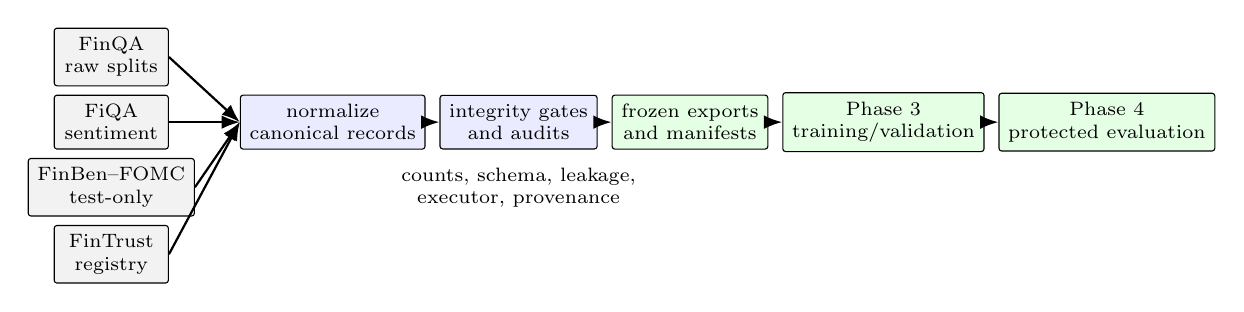
\begin{tikzpicture}[node distance=3pt and 5pt, >=Latex,
  source/.style={draw, rounded corners=1pt, fill=gray!10, align=center,
    minimum width=1.45cm, minimum height=0.62cm, font=\scriptsize},
  gate/.style={draw, rounded corners=1pt, fill=blue!8, align=center,
    minimum width=1.55cm, minimum height=0.62cm, font=\scriptsize},
  output/.style={draw, rounded corners=1pt, fill=green!10, align=center,
    minimum width=1.55cm, minimum height=0.62cm, font=\scriptsize},
  arrow/.style={->, thick}]
\node[source] (finqa) {FinQA\\raw splits};
\node[source, below=of finqa] (fiqa) {FiQA\\sentiment};
\node[source, below=of fiqa] (fomc) {FinBen--FOMC\\test-only};
\node[source, below=of fomc] (trust) {FinTrust\\registry};
\node[gate, right=9mm of fiqa] (normalize) {normalize\\canonical records};
\node[gate, right=of normalize] (checks) {integrity gates\\and audits};
\node[output, right=of checks] (exports) {frozen exports\\and manifests};
\node[output, right=of exports] (p3) {Phase 3\\training/validation};
\node[output, right=of p3] (p4) {Phase 4\\protected evaluation};
\draw[arrow] (finqa.east) -- (normalize.west);
\draw[arrow] (fiqa.east) -- (normalize.west);
\draw[arrow] (fomc.east) -- (normalize.west);
\draw[arrow] (trust.east) -- (normalize.west);
\draw[arrow] (normalize) -- (checks);
\draw[arrow] (checks) -- (exports);
\draw[arrow] (exports) -- (p3);
\draw[arrow] (p3) -- (p4);
\node[below=3pt of checks, align=center, font=\scriptsize] {counts, schema, leakage,\\executor, provenance};
\end{tikzpicture}
\caption{Phase-2.1 architecture. Raw benchmark sources are normalized into a shared record
contract, passed through integrity gates, and exported into explicit training, validation,
and protected-evaluation roles. FinBen--FOMC and FinTrust never enter the training pool.}
\label{fig:phase2-architecture}
\end{figure}

\subsection{Data contract and gate procedure}
The pipeline uses deterministic JSON serialization, a fixed seed of 42, and SHA-256
fingerprints for raw sources and exported artifacts. Gold evidence is retained as annotation
metadata but is excluded from model inputs. For FinQA, the official evaluator is run over
every gold program in every split and its result is compared with the official executable
answer. Leakage signatures hash normalized question, context, and table content; exact
cross-split collisions are hard failures. A MinHash-based near-duplicate audit compares
training records with protected tests and flags candidates for inspection rather than
silently deleting legitimate financial-report reuse.

\begin{figure}[t]
\centering
\begin{tikzpicture}[node distance=4pt and 6pt, >=Latex,
  step/.style={draw, rounded corners=1pt, fill=orange!10, align=center,
    minimum width=1.45cm, minimum height=0.7cm, font=\scriptsize},
  decision/.style={draw, diamond, aspect=2.0, fill=yellow!15, align=center,
    inner sep=1pt, font=\scriptsize}, arrow/.style={->, thick}]
\node[step] (raw) {raw data\\unchanged};
\node[step, right=of raw] (schema) {schema\\validation};
\node[step, right=of schema] (exec) {official\\execution};
\node[step, right=of exec] (leak) {leakage +\\near-duplicate};
\node[decision, right=8mm of leak] (pass) {ERROR gates\\pass?};
\node[step, right=8mm of pass] (freeze) {write\\FROZEN contract};
\draw[arrow] (raw) -- (schema);
\draw[arrow] (schema) -- (exec);
\draw[arrow] (exec) -- (leak);
\draw[arrow] (leak) -- (pass);
\draw[arrow] (pass) -- node[above, font=\scriptsize]{yes} (freeze);
\draw[arrow] (pass.south) |- node[pos=0.25, below, font=\scriptsize]{no: stop} (leak.south);
\end{tikzpicture}
\caption{Phase-2.1 gate lifecycle. Warnings remain visible in the validation report but do
not override a PASS when no ERROR-severity gate fails.}
\label{fig:phase2-gates}
\end{figure}

\begin{table}[t]
\centering
\caption{Phase-2.1 gate evidence and downstream roles.}
\label{tab:phase2-gates}
\small
\resizebox{\columnwidth}{!}{%
\begin{tabular}{p{0.24\columnwidth}p{0.28\columnwidth}p{0.38\columnwidth}}
\toprule
gate/evidence & observed result & downstream consequence\\
\midrule
split counts & FinQA 6,251/883/1,147; FiQA 822/117/234; FOMC 496 & fixed train, validation, and protected-test roles\\
schema and IDs & required fields present; 8,281 FinQA IDs unique & stable record interface\\
official execution & all FinQA gold programs execute and match executable answers & official executor required for model evaluation\\
exact leakage & zero cross-split full-input collisions & protected tests remain isolated\\
provenance & source and artifact SHA-256 manifests recorded & reproducible handoff\\
near duplicates & train--protected-test audit exported for inspection & warnings are reviewed, not silently removed\\
overall status & PASS; two non-blocking warnings & Phase 3/4 may proceed under frozen manifests\\
\bottomrule
\end{tabular}}
\end{table}

The Phase-2.1 validation report is a PASS with two explicit warnings: final-step annotation
agreement is 0.98261 (below the 0.99 warning threshold), and evaluator candidates were not
discovered for FinTrust dimensions trustfulness, safety, and privacy. These warnings do not
invalidate the FinQA/FiQA data contract, but the FinTrust gap remains a Phase-4 limitation.
The exported training pool contains 7,073 records (FinQA and FiQA only), while the validation
pool contains 1,000 records. The protected artifacts contain 1,147 FinQA test records, 234
FiQA test records, 496 FinBen--FOMC records, and the FinTrust registry.

\subsection{Phase-2.1 artifact and figure inventory}
Phase 2.1 produces integrity evidence rather than accuracy curves. The source paths and
hashes for the data registry, validation report, source fingerprints, official-execution
audit, near-duplicate audit, and downstream configuration manifests are listed in
\texttt{docs/phase2\_figure\_inventory.md}. The result plots used later in this
paper are therefore labeled as Phase-3 or Phase-4 plots, not Phase-2 plots: the former show
model baselines, and the latter show sampling, risk--coverage, and selection ablations.

\section{Method: \ourmethod{}}\label{sec:method}

\subsection{Sampling and execution verification}
Given $q$, sample $n$ programs $p^{(1)},\dots,p^{(n)}\sim\pi_{\theta}(\cdot\mid q)$
(temperature 0.7, top-$p$ 0.9, no other search). Each $p^{(i)}$ is run with the official
evaluator if it parses; an answer $a^{(i)}$ exists iff the program is valid and executes.
Evidence is carried by the \emph{candidate population}, not by any single decode.

\subsection{Trust features from the sample population}
For a question $q$ with $n$ candidates we compute three pre-registered features:
\begin{align}
  \mathcal{A}(q) &= \frac{1}{n(n-1)}\sum_{i\neq j}
    \mathbb{1}[a^{(i)} = a^{(j)}],\\
  \mathcal{R}(q) &= \frac{1}{n}\sum_{i=1}^{n} e^{(i)},\\
  e^{(i)} &= \mathbb{1}[p^{(i)}\ \text{valid}\ \wedge\ a^{(i)}\ \text{exists}],\\
  \mathcal{C}(q) &= \overline{\log\pi_{\theta}(p^{(\star)}\mid q)}.
\end{align}
where $p^{(\star)}$ is the selected candidate and the mean is over its tokens.
The feature vector is $f(q)=[\mathcal{A}(q),\,\mathcal{R}(q),\,\mathcal{C}(q)]$. The gold
answer is used only to \emph{score} these features, never to select a candidate or a
threshold (guardrail: nothing refit on test).

\subsection{Calibration (C2)}
The score $\p(q) = \Pr[\text{answer is correct} \mid f(q)]$ is learned by out-of-fold
Platt scaling:
\begin{equation}
  \p(q) \;=\; \sigma\!\big(w\cdot f(q) + b\big), \qquad
  \sigma(z) = \frac{1}{1+e^{-z}} ,
\end{equation}
with $(w,b)$ fit by logistic regression on inner-fold predictions and applied to outer folds
(5 folds), so every validation prediction is genuinely out-of-sample. Because a single-feature
monotone calibrator cannot reorder answers, we evaluate \textbf{(i)} a single-feature baseline
($f=[\mathcal{C}]$) and \textbf{(ii)} the full feature vector $f$ \textbf{(C3)}.

\subsection{Freeze and abstention rule (C2)}
For coverage target $1-\alpha$ (pre-registered $\alpha \in \{0.20, 0.10\}$):
\begin{equation}
\begin{aligned}
  \theta &= \min\{t : \CC_{\text{val}}(t) \ge 1-\alpha\},\\
  \CC(t) &= \frac{1}{|V|}\sum_{q\in V}\mathbb{1}[\p(q)\ge t].
\end{aligned}
\end{equation}
and the decision rule on any future question is answer $q$ iff $\p(q) \ge \theta$, else abstain.
Selective risk and coverage follow \citep{eliyaniv2010selective}:
\begin{equation}
\begin{aligned}
  \RR(\theta)&=\frac{\sum_q \ell(q)\,\mathbb{1}[\p(q)\ge\theta]}
                    {\sum_q\mathbb{1}[\p(q)\ge\theta]},\\
  \ell(q)&=\mathbb{1}[\text{answer}(q)\neq \text{gold}(q)].
\end{aligned}
\end{equation}

\begin{algorithm}[t]
\caption{\ourmethod{} decision pipeline (fit once on validation; frozen thereafter)}
\begin{algorithmic}[1]
\Require frozen adapter $\pi_\theta$, sampler params $(n,\tau,p)$, evaluator $\text{exec}$, coverage targets
\State \textbf{Validation phase:}
\For{$q \in V$}
  \State sample $n$ programs; keep valid ones; get answers $a^{(i)}$
  \State compute $f(q)=[\mathcal{A}(q),\,\mathcal{R}(q),\,\mathcal{C}(q)]$
\EndFor
\State fit out-of-fold Platt $w,b$ on $(f(q),\,\ell(q))_{q\in V}$; score $\p(q)$ OOF
\State pick $\theta$ s.t.\ $\CC_{\text{val}}(\theta) \ge 1-\alpha$ for each target
\State write \texttt{phase4\_freeze.json} (FROZEN, $w,b,\theta,\alpha$, sha256)
\State \textbf{Protected phase (opened once, after FROZEN + protected flag):}
\For{$q \in T$}
  \State draw $n$ candidates; if $\p(q) \ge \theta$ emit answer$(q)$, else \textbf{abstain}
\EndFor
\end{algorithmic}
\end{algorithm}

\section{Experimental setup}\label{sec:setup}
\paragraph{Data and aligned evaluation.}
FinQA (train 6\,251 / validation 883 / held-out test 1\,147) uses the official program
evaluator; we report three aligned accuracies: \emph{printed} (the answer string the model
emits), \emph{program} (does the parse succeed), and \emph{execution} (does the executed
answer match gold). FiQA (validation 117 / test 234) is regression with MAE, $R^2$,
Pearson $r$ at tolerance 0.10. FOMC (test 496: neutral 245, dovish 129, hawkish 122) is
zero-shot stance classification with accuracy, macro-F1 and parse success.
The datasets do not provide reliable participant demographics such as age or gender;
therefore this study reports no inferred demographic distribution. The records are treated
as financial-document and sentiment annotations, not as a human-subject sample. This
distinction prevents demographic claims from being inferred from names, writing style, or
model outputs.
\paragraph{Data contract and split policy.}
The Phase-2.1 contract fixes the dataset roles before training. FinQA and FiQA training
partitions may enter the training pool; validation partitions support model selection; and
the FinQA and FiQA tests, FinBen-FOMC, and FinTrust resources remain protected. Source
fingerprints are recorded with SHA-256 manifests, canonical serialization is used for
structured records, and exact-overlap audits compare normalized input signatures rather
than relying only on record identifiers. Near-duplicate candidates are flagged for manual
inspection rather than silently removed, since financial reports can legitimately reuse
standard language. These controls establish provenance and split isolation, not semantic
correctness of every annotation.

\begin{table}[t]
\centering
\caption{Dataset roles and split sizes fixed by the Phase-2.1 contract.}
\label{tab:data-contract}
\small
\resizebox{\columnwidth}{!}{%
\begin{tabular}{lrrrr}
\toprule
dataset & train & validation & test & role\\
\midrule
FinQA & 6\,251 & 883 & 1\,147 & numerical reasoning\\
FiQA & 822 & 117 & 234 & sentiment regression\\
FinBen-FOMC & 0 & 0 & 496 & external stance evaluation\\
FinTrust & -- & -- & protected & trust evaluation\\
\bottomrule
\end{tabular}}
\end{table}
\paragraph{Model.} Frozen Phase-3 winner: \texttt{Qwen/Qwen3-1.7B}
\citep{qwen2025qwen3} with balanced-joint QLoRA \citep{dettmers2023qlora} as canonical on
FinQA and explicit-schema on FiQA; exact hyper-parameters are in
\texttt{phase3\_freeze.json} and were fixed before this work began.
\paragraph{Metrics.} Brier, ECE-10, expected AURC (e-AURC; lower is better), coverage and
selective risk. All numbers cited as ``validation'' are out-of-fold or tuned on
validation; all ``test'' numbers were produced by the frozen system and are unchanged since
the completed protected run (see \texttt{docs/exp\_4(b).md}).

\begin{table}[t]
\centering
\caption{Validation baseline matrix. These values are development results and are not
protected-test measurements. E8 is a secondary model-family comparison, not a controlled
architecture comparison.}
\label{tab:validation-baselines}
\small
\resizebox{\columnwidth}{!}{%
\begin{tabular}{l l r r r r}
\toprule
ID & configuration & FinQA exec. & program & answer & FiQA MAE / $R^2$\\
\midrule
E1 & Qwen3 zero-shot & 0.000 & 0.000 & 0.005 & 0.501 / -1.787\\
E2 & Qwen3 few-shot & 0.000 & 0.000 & 0.000 & 0.185 / 0.472\\
E3 & Qwen3 FinQA-only QLoRA & 0.681 & 0.624 & 0.390 & 0.505 / -1.840\\
E4 & Qwen3 FiQA-only QLoRA & 0.000 & 0.000 & 0.000 & 0.129 / 0.725\\
E5 & Qwen3 joint balanced QLoRA & 0.675 & 0.612 & 0.376 & 0.130 / 0.730\\
E8 & Phi joint balanced QLoRA & 0.701 & 0.640 & 0.386 & 0.130 / 0.809\\
E11 & Qwen3 joint natural sampling & 0.615 & 0.555 & 0.344 & 0.128 / 0.736\\
\bottomrule
\end{tabular}}
\end{table}

\begin{table}[t]
\centering
\caption{\label{tab:c1} C1 evidence. \textbf{(top)} FinQA held-out test, execution accuracy
per rule ($n{=}8$); \textbf{(bottom)} FiQA test regression. EVG neither beats nor loses to
the frozen greedy baseline on either task; per-record, 18 questions are won and 20 lost.}
\small
\begin{tabular}{lc}
\toprule
\multicolumn{2}{l}{\emph{FinQA test, execution accuracy ($n{=}1147$)}}\\
\midrule
frozen greedy (baseline) & \textbf{0.6574}\\
candidate-0 (prints) & 0.6399\\
self-consistency vote & 0.6478\\
best-of-$n$ & 0.6556\\
\textbf{execution-verified (ours)} & 0.6556\\
\bottomrule
\end{tabular}
\vspace{0.5em}
\resizebox{\columnwidth}{!}{%
\begin{tabular}{lcc}
\toprule
\multicolumn{3}{l}{\emph{FiQA test ($n{=}234$), MAE / accuracy@0.10}}\\
\midrule
frozen greedy & \textbf{0.1301} & \textbf{0.568}\\
median-of-$n$ (ours) & 0.1306 & 0.556\\
\bottomrule
\end{tabular}}
\end{table}

\begin{figure}[t]
\centering
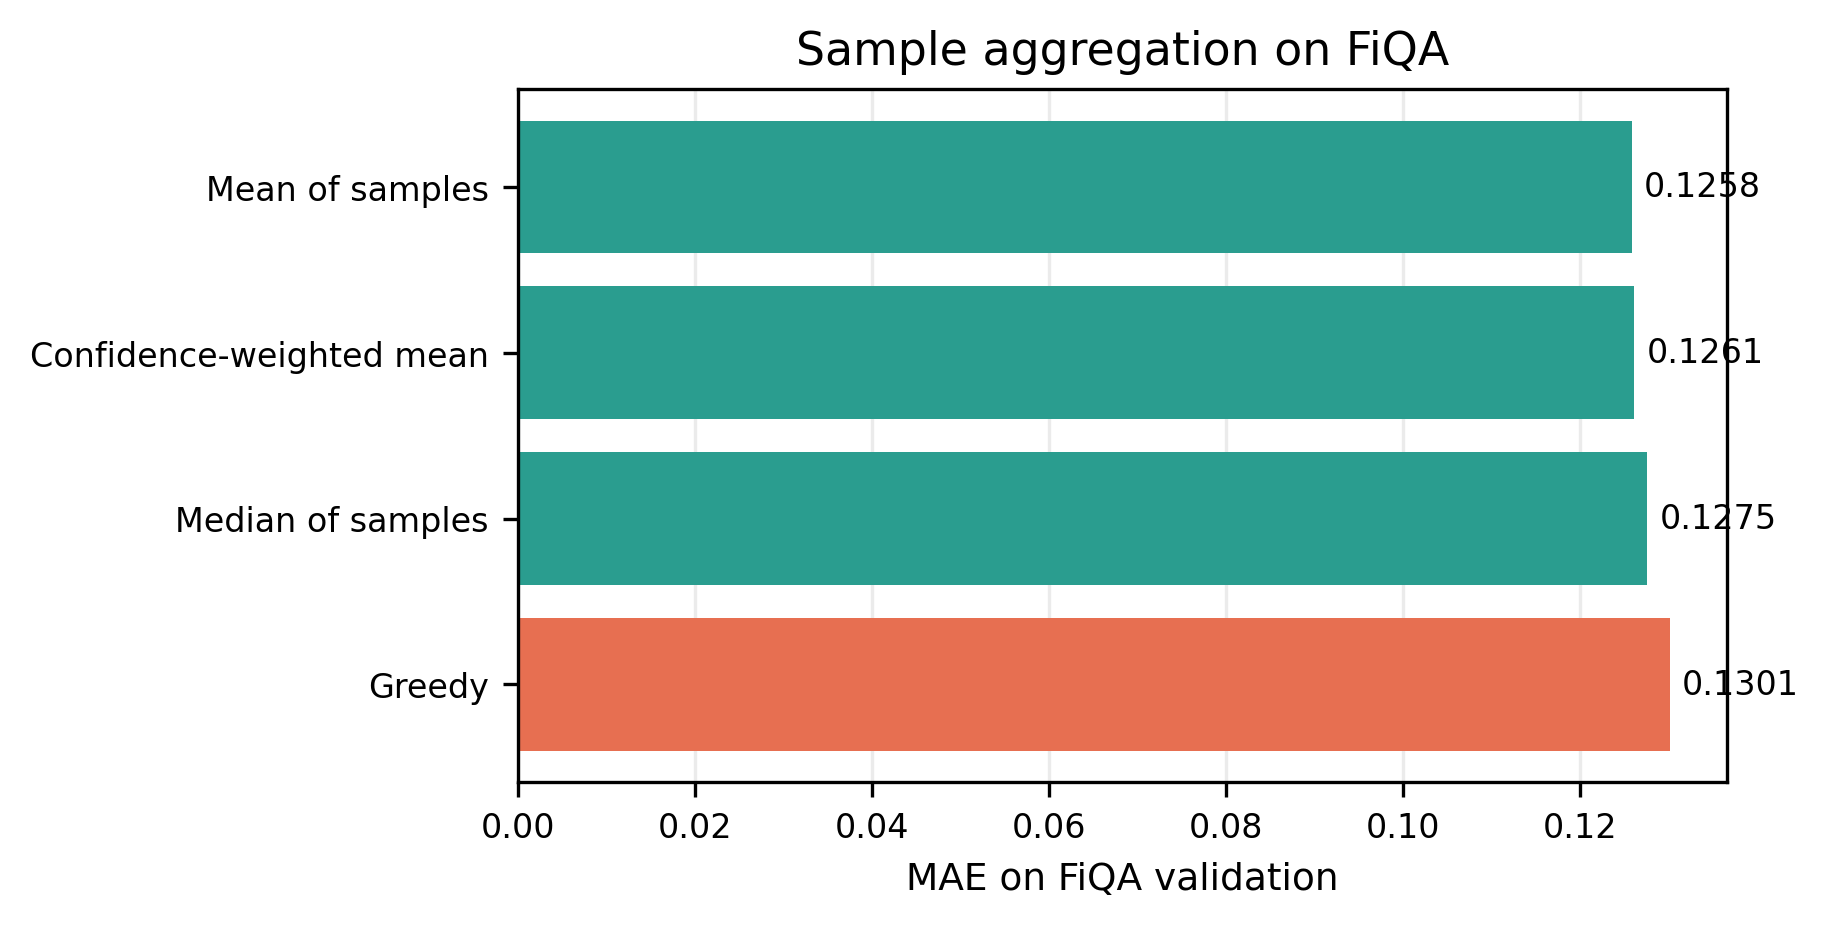
\includegraphics[width=\linewidth]{fig_phase4_fiqa_aggregation.png}
\caption{FiQA validation aggregation over sampled predictions. Lower MAE is better;
median and mean aggregation improve on greedy decoding in this validation diagnostic,
while the frozen protected-test policy remains the pre-registered greedy baseline.}
\label{fig:fiqa-sampling}
\end{figure}

\begin{table}[t]
\centering
\caption{\label{tab:agreement} Agreement bins vs.\ correctness on the protected test.
Agreement is steeply and monotonically predictive, while the model's log-probability cannot
separate correct from incorrect answers (ROC-AUC 0.58).}
\small
\begin{tabular}{lcc}
\toprule
EVG agreement bin & $n$ records & execution accuracy\\
\midrule
(0.00, 0.25] & 35 & \textbf{0.029}\\
(0.25, 0.50] & 122 & 0.238\\
(0.50, 0.75] & 181 & 0.448\\
(0.75, 1.00] & 809 & \textbf{0.792}\\
\bottomrule
\end{tabular}
\end{table}

\begin{figure}[t]
\centering
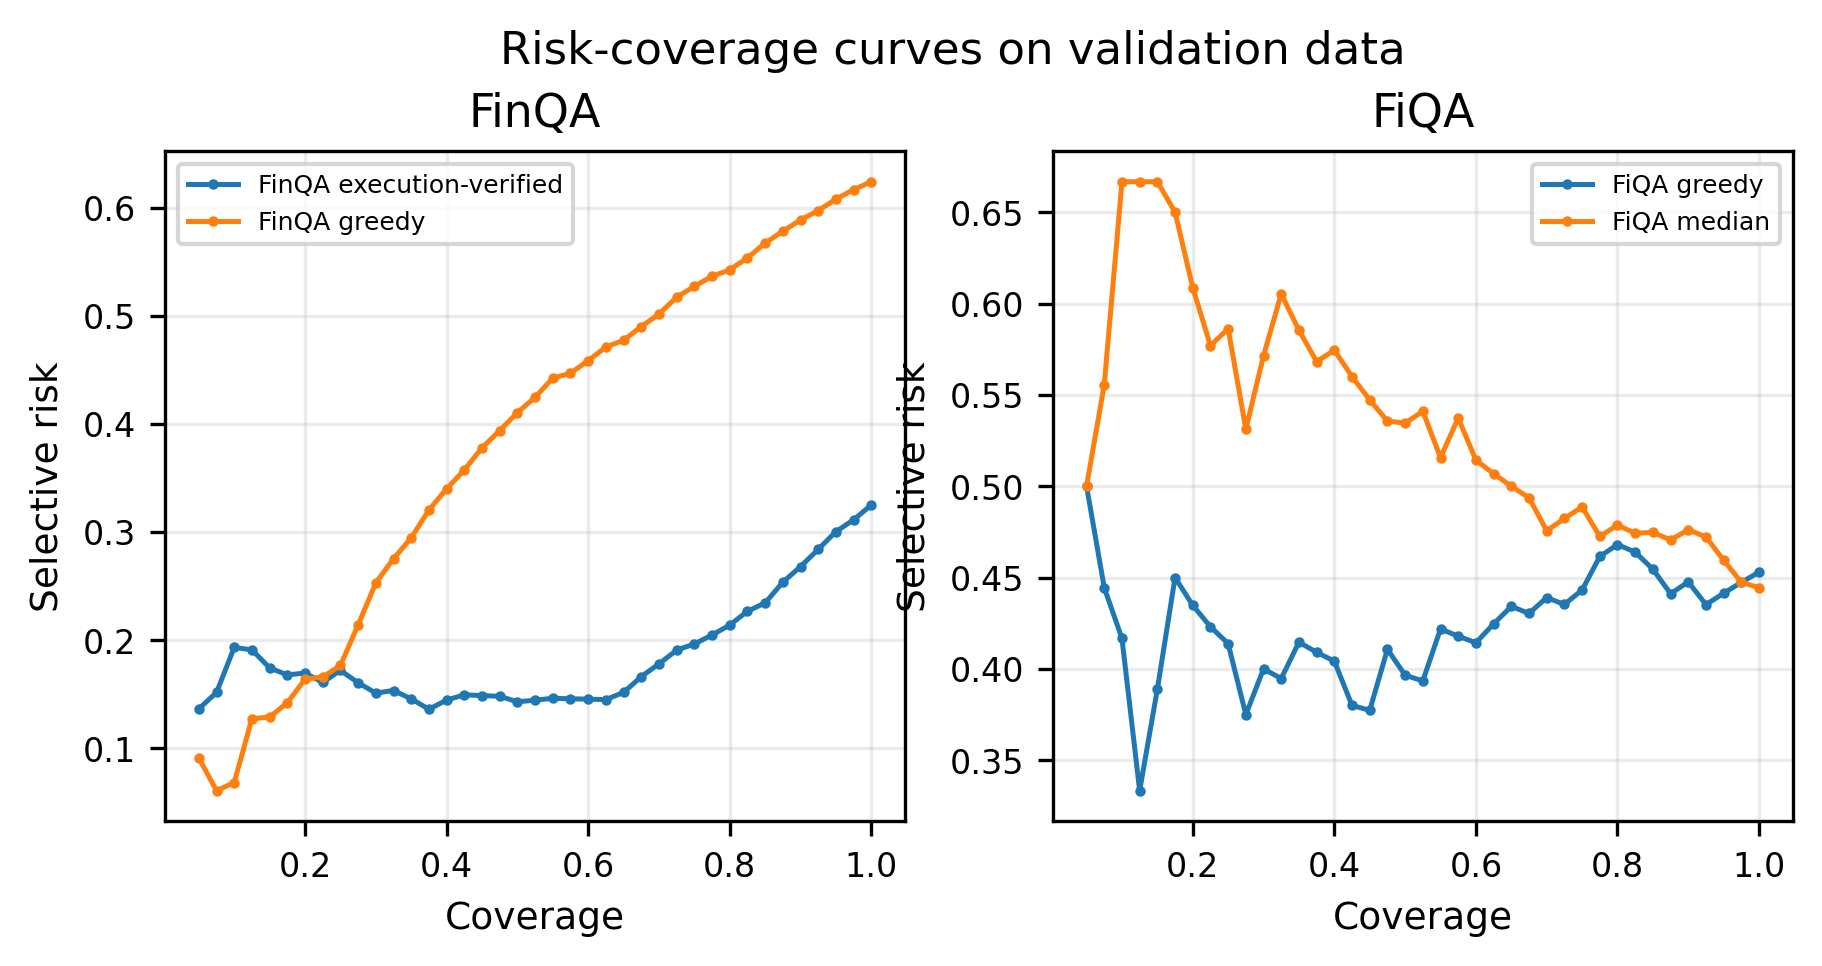
\includegraphics[width=\linewidth]{fig_phase4_risk_coverage.png}
\caption{Out-of-fold risk--coverage curves for FinQA and FiQA validation. The calibrated
FinQA execution-verified policy lowers selective risk as coverage is reduced; FiQA shows
weaker separation, consistent with its small regression validation split.}
\label{fig:risk-coverage}
\end{figure}

\begin{table}[t]
\centering
\caption{\label{tab:calib} C2/C3 calibration results on FinQA validation (out-of-fold).
\emph{Top:} ordering quality (e-AURC, lower better). Single-feature calibrators do not move
the raw ranking (a monotone map cannot); the agreement-driven full vector does ($-$39.3\%).
\emph{Bottom:} probability quality of the frozen policy.}
\small
\resizebox{\columnwidth}{!}{%
\begin{tabular}{lcc}
\toprule
\multicolumn{3}{l}{\emph{e-AURC on FinQA validation (frame = exec-verified)}}\\
\midrule
raw confidence & 0.2029\\
+ isotonic (feature: confidence) & 0.2028\\
+ Platt (feature: confidence) & 0.2496\\
\rowcolor{gray!15} \textbf{+ Platt (features: agree, exec, conf)} & \textbf{0.1232}\\
\multicolumn{3}{l}{\quad baseline greedy frame, best method: 0.1897}\\
\midrule
\multicolumn{3}{l}{\emph{Probability quality (frozen FinQA policy)}}\\
\midrule
raw confidence / Platt full & Brier 0.2845~$\rightarrow$~\textbf{0.1579} & ECE 0.2555~$\rightarrow$~\textbf{0.0475}\\
\bottomrule
\end{tabular}}
\end{table}

\begin{figure}[t]
\centering
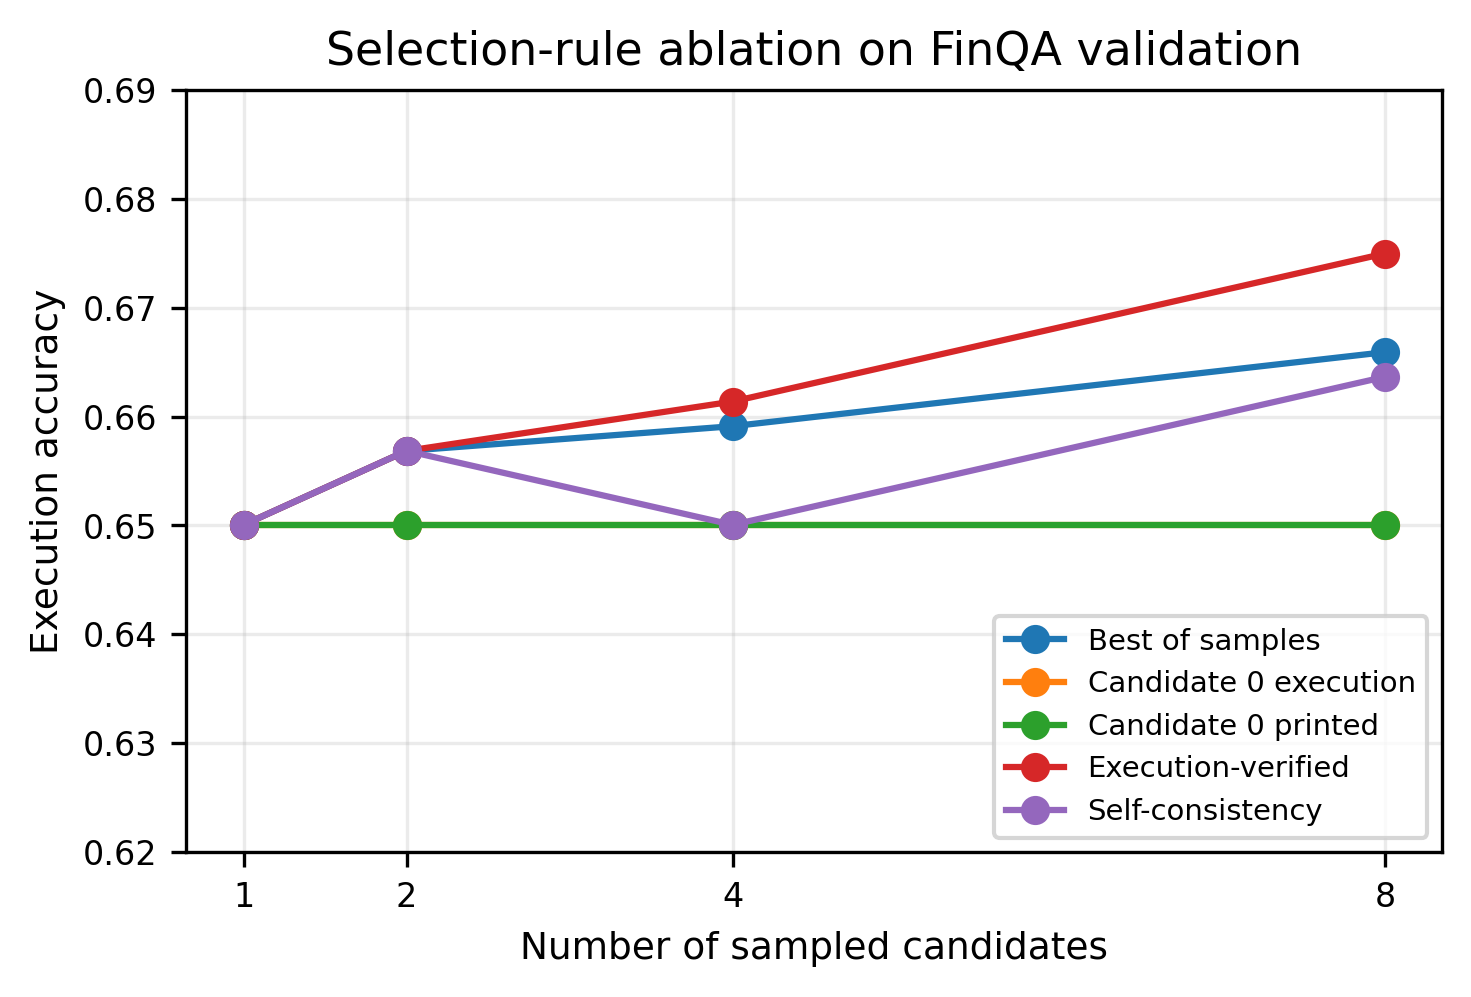
\includegraphics[width=\linewidth]{fig_phase4_selection_ablation.png}
\caption{FinQA validation ablation over the number of sampled candidates. The horizontal
lines show the frozen greedy answer and executor baselines; execution-verified selection
does not produce a protected-test accuracy gain, motivating its use as a selective-risk
signal rather than as an accuracy claim.}
\label{fig:selection-ablation}
\end{figure}

\begin{table}[t]
\centering
\caption{\label{tab:transfer} Transferred abstention (frozen thresholds, protected test).
The threshold and calibration were fixed on validation \emph{before} the test opened; the
realised behaviour is close to predicted ($-$31.0\% vs\ $-$34.2\%). FiQA, as pre-frozen on
raw confidence, abstains to no effect ($-$2.9\%).}
\small
\resizebox{\columnwidth}{!}{%
\begin{tabular}{lcccccc}
\toprule
\multicolumn{7}{l}{\emph{FinQA (frozen: exec-verified + Platt-full + $\theta$)}}\\
\toprule
target & $\theta$ & test cov. & select. risk & selected acc. & abstained & err.\ rel.\ $\Delta$\\
\midrule
0.80 & 0.409 & 0.786 & \textbf{0.2375} & \textbf{0.7625} & 246 & \textbf{$-$31.0\%}\\
0.90 & 0.221 & 0.926 & 0.3004 & 0.6996 & 85 & $-$12.8\%\\
\bottomrule
\end{tabular}}
\vspace{0.4em}
\resizebox{\columnwidth}{!}{%
\begin{tabular}{lcccc}
\toprule
\multicolumn{5}{l}{\emph{FiQA (frozen: greedy + raw confidence)}}\\
\toprule
target & test cov. & select. risk & full risk & err.\ rel.\ $\Delta$\\
\midrule
0.80 & 0.765 & 0.4190 & 0.4316 & $-$2.9\%\\
0.90 & 0.885 & 0.4203 & 0.4316 & $-$2.6\%\\
\bottomrule
\end{tabular}}
\end{table}

\begin{table}[t]
\centering
\caption{\label{tab:rigor} Evaluation rigor on the protected test (n=1,147). \textbf{(top)}
Paired comparison: the C1 tie is statistically verified, not read off rounded means.
\textbf{(middle)} Error taxonomy: the only channel EVG fails to fix is the \emph{printed}
answer string. \textbf{(bottom)} Reasoning-depth stratification: abstention concentrates on
the deepest programs and delivers its largest relative gain there. Bootstrap CI: 10{,}000
resamples; McNemar exact (binomial).}
\small
\begin{tabular}{lcc}
\toprule
\multicolumn{3}{l}{\emph{C1 significance (protected test, paired)}}\\
\toprule
 & greedy & exec-verified\\
\midrule
execution acc. & 0.6574 & 0.6556\\
delta & \multicolumn{2}{c}{$-0.0017$ \quad 95\% CI $[-0.0122,\,+0.0087]$}\\
McNemar exact $p$ & \multicolumn{2}{c}{0.871}\\
\bottomrule
\end{tabular}
\vspace{0.6em}
\resizebox{\columnwidth}{!}{%
\begin{tabular}{lrr}
\toprule
\multicolumn{3}{l}{\emph{Error taxonomy (mutually exclusive; partitions sum to 1,147)}}\\
\toprule
cell (greedy) & $n$ & \% \\
\midrule
parse failure & 0 & 0.0\\
invalid / unexecutable program & 3 & 0.3\\
exec.\ correct \& print correct & 399 & 34.8\\
exec.\ correct \& print wrong (format mismatch) & 355 & 31.0\\
exec.\ wrong \& print wrong & 388 & 33.8\\
exec.\ wrong \& print correct & 2 & 0.2\\
\midrule
\emph{exec-verified:} invalid / executes-wrong / correct & 0 / 395 / 752 & ---\\
\bottomrule
\end{tabular}}
\vspace{0.6em}
\resizebox{\columnwidth}{!}{%
\begin{tabular}{lrrrr}
\toprule
program ops & $n$ & full acc. & selected acc. & err.\ $\Delta$\\
\midrule
0 & 45 & 0.844 & 0.884 & $-$25.2\%\\
1 & 644 & 0.649 & 0.764 & $-$32.6\%\\
2 & 391 & 0.662 & 0.748 & $-$25.2\%\\
3--6 & 67 & 0.552 & 0.739 & $-$41.7\%\\
\bottomrule
\end{tabular}}
\end{table}

\begin{table}[t]
\centering
\caption{\label{tab:fomc} Zero-shot out-of-domain robustness on FinBen-FOMC (test, 496):
the frozen financial adapter improves the balanced metric and the rare classes that a
neutral-majority model otherwise ignores.}
\small
\resizebox{\columnwidth}{!}{%
\begin{tabular}{lcccccc}
\toprule
system & accuracy & macro-F1 & parse & F1 dovish & F1 neutral & F1 hawkish\\
\midrule
base \texttt{Qwen/Qwen3-1.7B} & 0.454 & 0.215 & 0.899 & 0.163 & 0.650 & 0.046\\
\textbf{+ frozen E5 adapter} & 0.484 & \textbf{0.304} & \textbf{0.986} & 0.333 & 0.621 & 0.260\\
\bottomrule
\end{tabular}}
\end{table}

\begin{table}[t]
\centering
\caption{\label{tab:ablate} Abstention strategies compared at \emph{matched} coverage on the
protected test (n=1,147; each strategy answers the same $k{=}\lfloor\mathtt{cov}\cdot n\rfloor$
questions, ranked by its own score, evaluated on the execution channel). Confidence-based
abstention of the greedy baseline is a weak tool ($\le$8\%); agreement ranks and abstains,
cutting answered-error 29.7\% at 80\% coverage. Ablation (right): agreement is necessary and
sufficient.}
\small
\resizebox{\columnwidth}{!}{%
\begin{tabular}{lccc}
\toprule
strategy (ranking score) & cov 0.5 & cov 0.8 & cov 0.9\\
\midrule
greedy + confidence & 0.674 & 0.685 & 0.677\\
best-of-8 + confidence & 0.660 & 0.654 & 0.659\\
exec-verified + agreement & \textbf{0.818} & \textbf{0.758} & \textbf{0.715}\\
exec-verified + agreement$\cdot$executability & 0.818 & 0.758 & 0.714\\
exec-verified + frozen $\hat p$ & 0.818 & 0.754 & 0.710\\
\bottomrule
\end{tabular}}
\vspace{0.6em}
\resizebox{\columnwidth}{!}{%
\begin{tabular}{lccc}
\toprule
config & agreement & executab. & confidence\\
\midrule
A & -- & -- & \checkmark \quad risk 0.315\\
B & \checkmark & -- & -- \quad \textbf{0.242}\\
C & -- & \checkmark & \checkmark \quad $\approx$ A\\
D & \checkmark & \checkmark & -- \quad 0.242\\
E (full) & \checkmark & \checkmark & \checkmark \quad 0.246\\
\bottomrule
\end{tabular}}
\end{table}

\section{Results}\label{sec:results}
\paragraph{C1 is rejected --- and that is a result.}
Table~\ref{tab:c1} and Figure~\ref{fig:fiqa-sampling}. On the protected test, execution-verified selection is 0.6556 vs.\
frozen greedy 0.6574 ($-$0.18~pp; per-record 18 gained, 20 lost, exact McNemar $p=0.871$,
bootstrap 95\% CI $[-0.0122,+0.0087]$), and the FiQA median-based
aggregator is 0.0005 worse in MAE. Validation showed the same story (tie: 0.6750 vs.\ 0.6750).
The one clean C1 win is \emph{program hygiene}: the invalid-program rate in the emitted
answers drops from $3.5\times10^{-3}$ to exactly \textbf{0}. Every answer we keep is backed
by a program the official evaluator accepted. On FiQA the median-of-8 aggregator also
betters neither MAE nor coverage; at matched coverage its \emph{ranking} is nevertheless the
best of the tested scores (selective MAE 0.1094 vs.\ 0.1176 for greedy-confidence at 80\%
coverage, n=234) --- a descriptive, small-sample hint that agreement transfers as a ranking
signal to regression too (see \S~matched coverage, below).

\paragraph{Agreement is the trust signal (C3 evidence at the decision level).}
Table~\ref{tab:agreement}. On protected data the model reports total
\emph{disagreement} (agreement $\le 0.25$) on records that are 2.9\% correct and unanimous
agreement (the top bin, $0.75$--$1.0$) on records that are 79.2\% correct; nothing in the
model's own log-probability separates these regimes (ROC-AUC 0.58 vs.\ 0.76 for agreement).
This is the signal that buys abstention.

\paragraph{Calibration gives the threshold meaning (C2).}
Table~\ref{tab:calib}. Out-of-fold Platt on the agreement features cuts Brier 0.28
$\rightarrow$ 0.16 and ECE 0.26 $\rightarrow$ 0.05. The ranking result is exactly what the
monotonicity caveat predicts: the single-feature calibrators cannot move e-AURC
(0.2029 $\rightarrow$ 0.2028), while the agreement-driven vector drops it to 0.1232
($-$39.3\% vs.\ raw, $-$35.1\% vs.\ the best baseline frame).

\paragraph{The frozen policy transfers (C2's operational payoff).}
Table~\ref{tab:transfer} and Figure~\ref{fig:risk-coverage}. With the threshold fixed on validation, opening the protected test
once yields: coverage 0.786 at the 0.80 target, selective risk 0.2375 (accuracy 0.7625)
vs.\ 0.3444 at full coverage --- a \textbf{31.0\% relative error reduction}, against the
34.2\% predicted from validation; bootstrap 95\% CI on the reduction is $[22.8\%,\,39.3\%]$
(i.e.\ the transfer is significant, not a rounding effect). FiQA abstention is -2.9\%: as the frozen FiQA method (raw
confidence on greedy) predicted, its errors are not rankable.

\paragraph{Rigor, error taxonomy, and depth (Table~\ref{tab:rigor}).}
The protected test was opened once against the frozen manifest. Per-record significance
testing formalises the C1 verdict; the remaining error is not parsing (0/1,147) and --
for EVG -- not program validity (0/1,147), but 395 genuine arithmetic slips (34.4\%).
The taxonomy uses mutually exclusive cells that sum to $n$: for greedy, 3 invalid
programs, 388 execute-and-print-wrong, 355 \emph{format mismatches} (the executed value is
correct but the printed string differs), and 2 cases where the printed string matches gold
while the executed value differs. Execution accuracy ($0.6574$) and printed-answer accuracy
($0.3496$) therefore differ \emph{solely} by the 355-record format channel; EVG's
\texttt{exec\_verified} rule removes that channel by construction. Stratifying by the FinQA
program-depth proxy, the frozen policy abstains least on 0-op lookups (4.4\%) and most on
3--6-op programs (31.3\%), where it cuts error by 41.7\%: abstention cost is spent precisely
where reasoning is deepest. All numbers carry bootstrap CIs in the annexed rigor report; the
calibration threshold used here was frozen on validation and never touched after the test
opened.

\paragraph{The mechanism survives comparison at matched coverage (Table~\ref{tab:ablate}).}
Figure~\ref{fig:selection-ablation} shows the corresponding validation ablation. Review pressure asks how agreement-abstention compares with standard alternatives when
they answer the \emph{same number of questions}. Table~\ref{tab:ablate} selects $k =
\lfloor \mathtt{cov}\cdot 1147\rfloor$ records by each score and measures selective risk on
the execution channel. Confidence-only abstention of the greedy baseline buys almost nothing
($\le$8\% error reduction; ROC-AUC 0.578) and best-of-n selection slightly hurts; ranking by
agreement alone cuts error 29.7\% vs.\ greedy-full and $-$23\% vs.\ a confidence-abstainer at
the same coverage. A paired bootstrap (B=3{,}000) on the risk difference at coverage 0.80
gives $[-0.093,\,-0.055]$ with $P=1.0$ against the confidence baseline. The leaving-one-out
ablation is sharp: agreement is necessary and sufficient; the executability feature is
uninformative (AUC 0.51) and the frozen Platt vector adds no ranking over agreement
($P{=}0.097$), though it supplies the pre-registered threshold its probability meaning.

\paragraph{Out-of-domain robustness.}
Table~\ref{tab:fomc}. Without any FOMC data in training, the frozen adapter raises macro-F1
0.21 $\rightarrow$ 0.30 and parse success 0.90 $\rightarrow$ 0.99, with the gain in the
rare classes (dovish F1 0.16 $\rightarrow$ 0.33; hawkish 0.05 $\rightarrow$ 0.26).

\paragraph{Cost.} EVG at $n=8$ runs at 4.8~s/question vs.\ 1.3~s greedy (3.7$\times$,
shared prefill), peak VRAM 3.1~GB / 6~GB. The offered trade is therefore 31\% fewer
answered errors at $\approx$80\% coverage in exchange for 3.7$\times$ latency on a laptop-class
model; whether that is \emph{worth} it is a deployment decision, not a claim we make.

\section{Additional Validation Diagnostics}
\label{sec:diagnostics}
The protected-test analysis establishes the paper's main selective-prediction result, while
the Phase-3 validation artifacts provide a more granular view of how the adapted model
fails. We report these diagnostics separately because they were available during model
development and therefore cannot be treated as additional protected-test evidence.

\subsection{Failure channels}
The E5 validation export separates execution correctness, program validity, and printed
answer correctness. The corresponding rates are 0.6750, 0.6116, and 0.3760, with an
invalid-program rate of $3/883=0.0034$. The gap between execution and printed accuracy is
not a contradiction: a program can execute to the correct numerical value while the
emitted answer string differs in formatting. This is why the protected analysis reports
the execution and printed channels independently. Figure~\ref{fig:validation-failures}
summarizes the audited validation failure categories; it is a diagnostic of E5 validation,
not a replacement for the protected-test taxonomy in Table~\ref{tab:rigor}.

\begin{figure}[t]
\centering
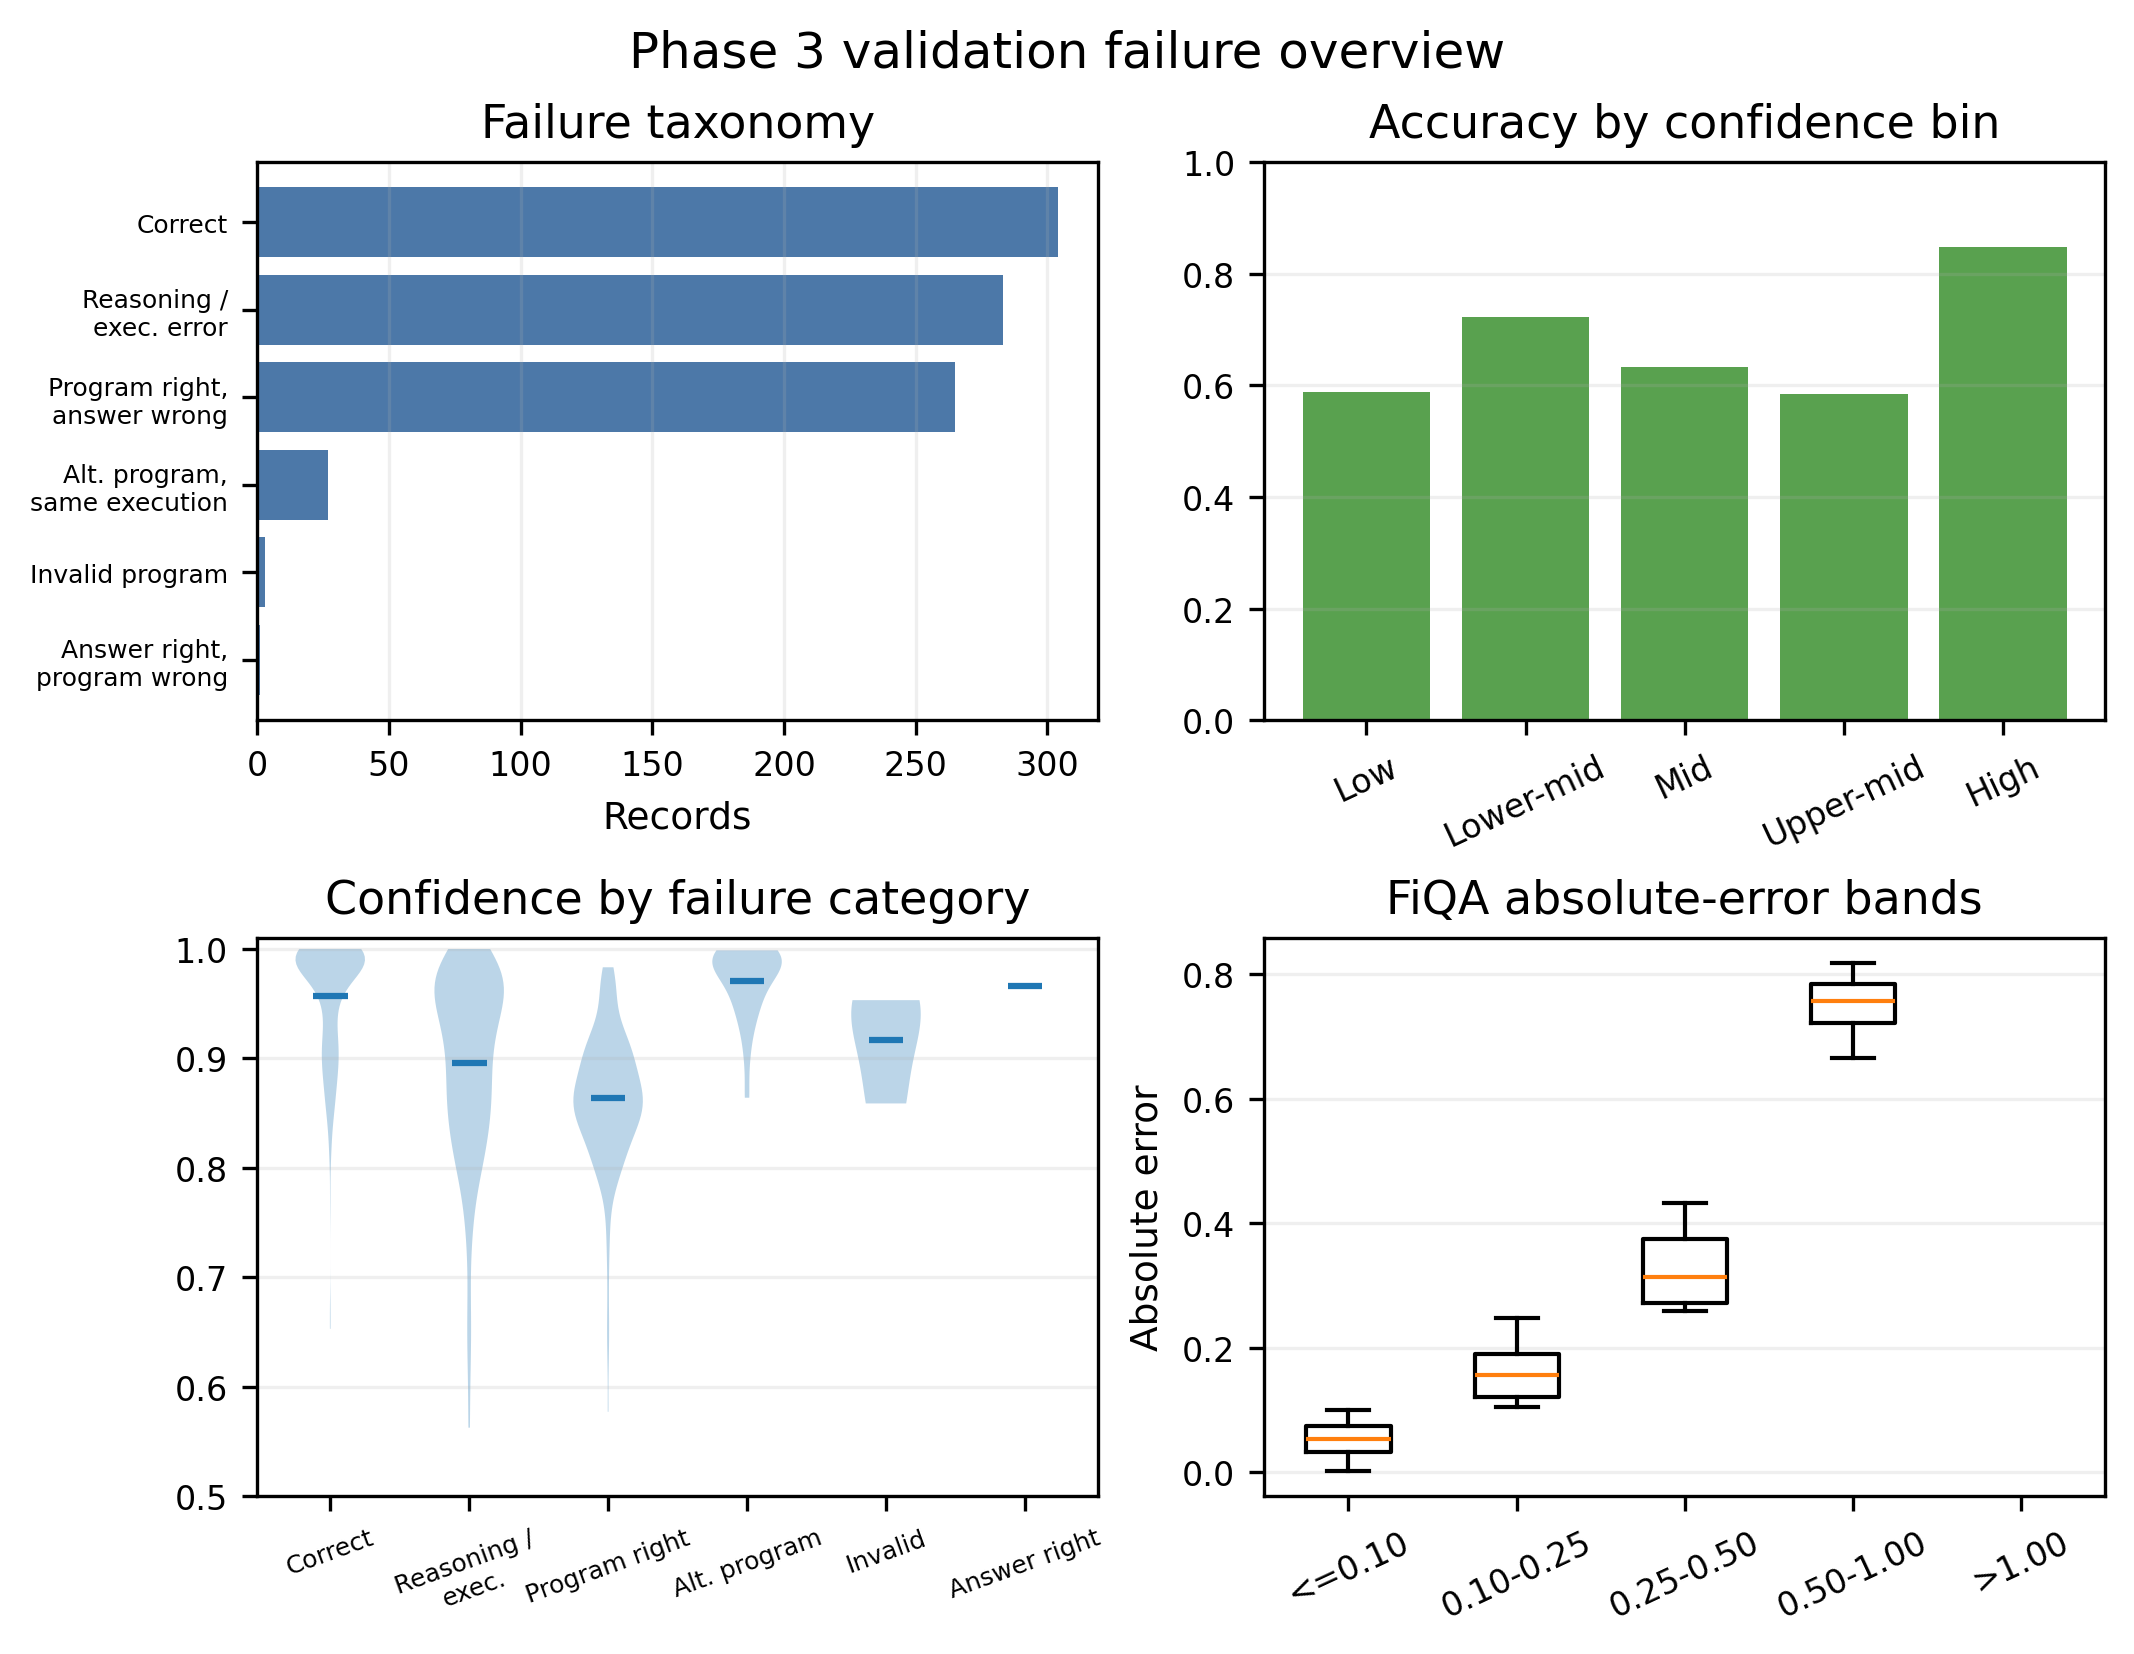
\includegraphics[width=\linewidth]{fig6_finqa_failure_overview.png}
\caption{E5 validation failure overview generated from the Phase-3 analysis artifacts.
Execution, program, and printed-answer channels are kept distinct.}
\label{fig:validation-failures}
\end{figure}

\subsection{Confidence and error magnitude}
The initial token-confidence diagnostic was intentionally conservative: a Spearman
correlation of 0.125 and ROC-AUC of 0.577 do not establish calibrated probabilities.
Confidence bins also show that a model can assign similar token likelihoods to correct and
incorrect numerical responses. Figure~\ref{fig:confidence-failures} visualizes the
relationship between confidence and failure category in the validation export. The later
EVG-CAS study therefore uses agreement among executed candidates as a separate feature,
then calibrates it out-of-fold rather than interpreting raw token likelihood as a risk
probability.

\begin{figure}[t]
\centering
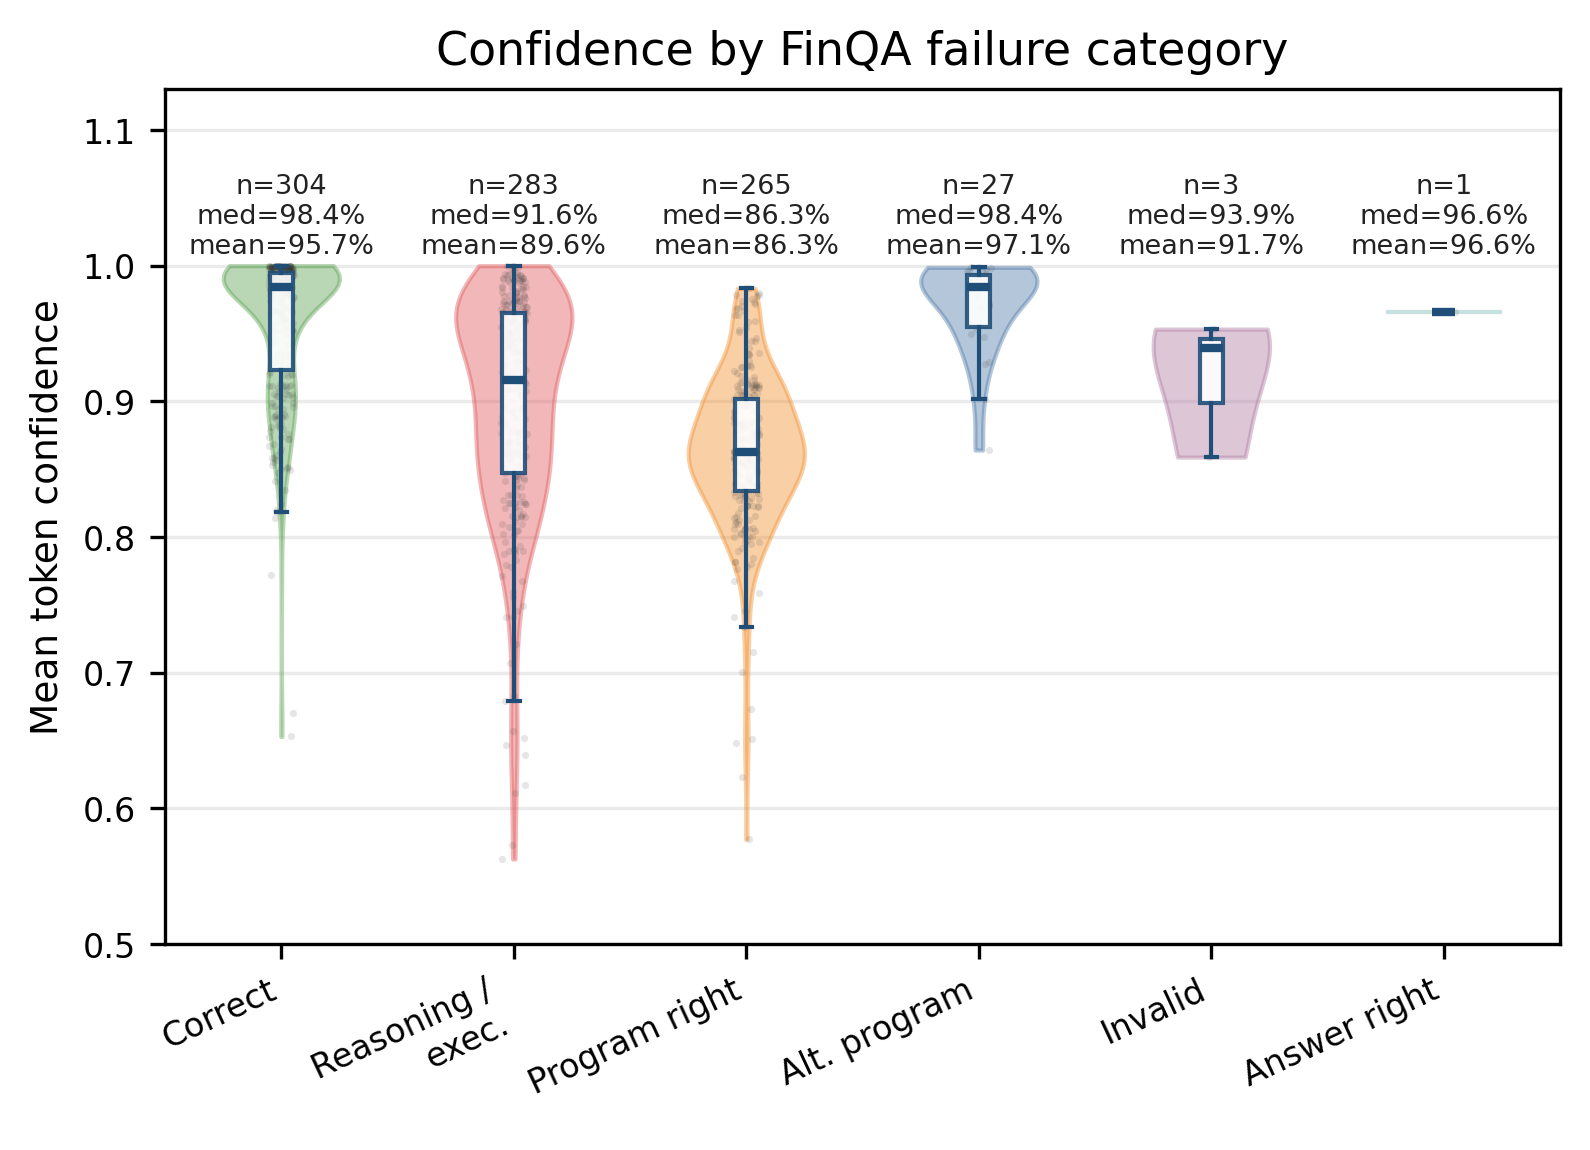
\includegraphics[width=\linewidth]{fig3_finqa_confidence_by_failure.png}
\caption{E5 validation confidence by FinQA failure category. Individual observations,
box summaries, medians, means, and category counts are shown. Raw generation confidence is
not used as a calibrated probability without validation-only calibration.}
\label{fig:confidence-failures}
\end{figure}

FiQA requires a different error interpretation because its target is continuous. The E5
validation MAE is 0.1301 and $R^2$ is 0.7301, but aggregate scores do not reveal whether
errors concentrate at the positive or negative ends of the sentiment scale. Figure~\ref{fig:fiqa-errors}
shows the absolute-error distribution used for this inspection. The small validation size
($n=117$) means that these patterns should be treated as descriptive rather than as
population-level estimates.

\begin{figure}[t]
\centering
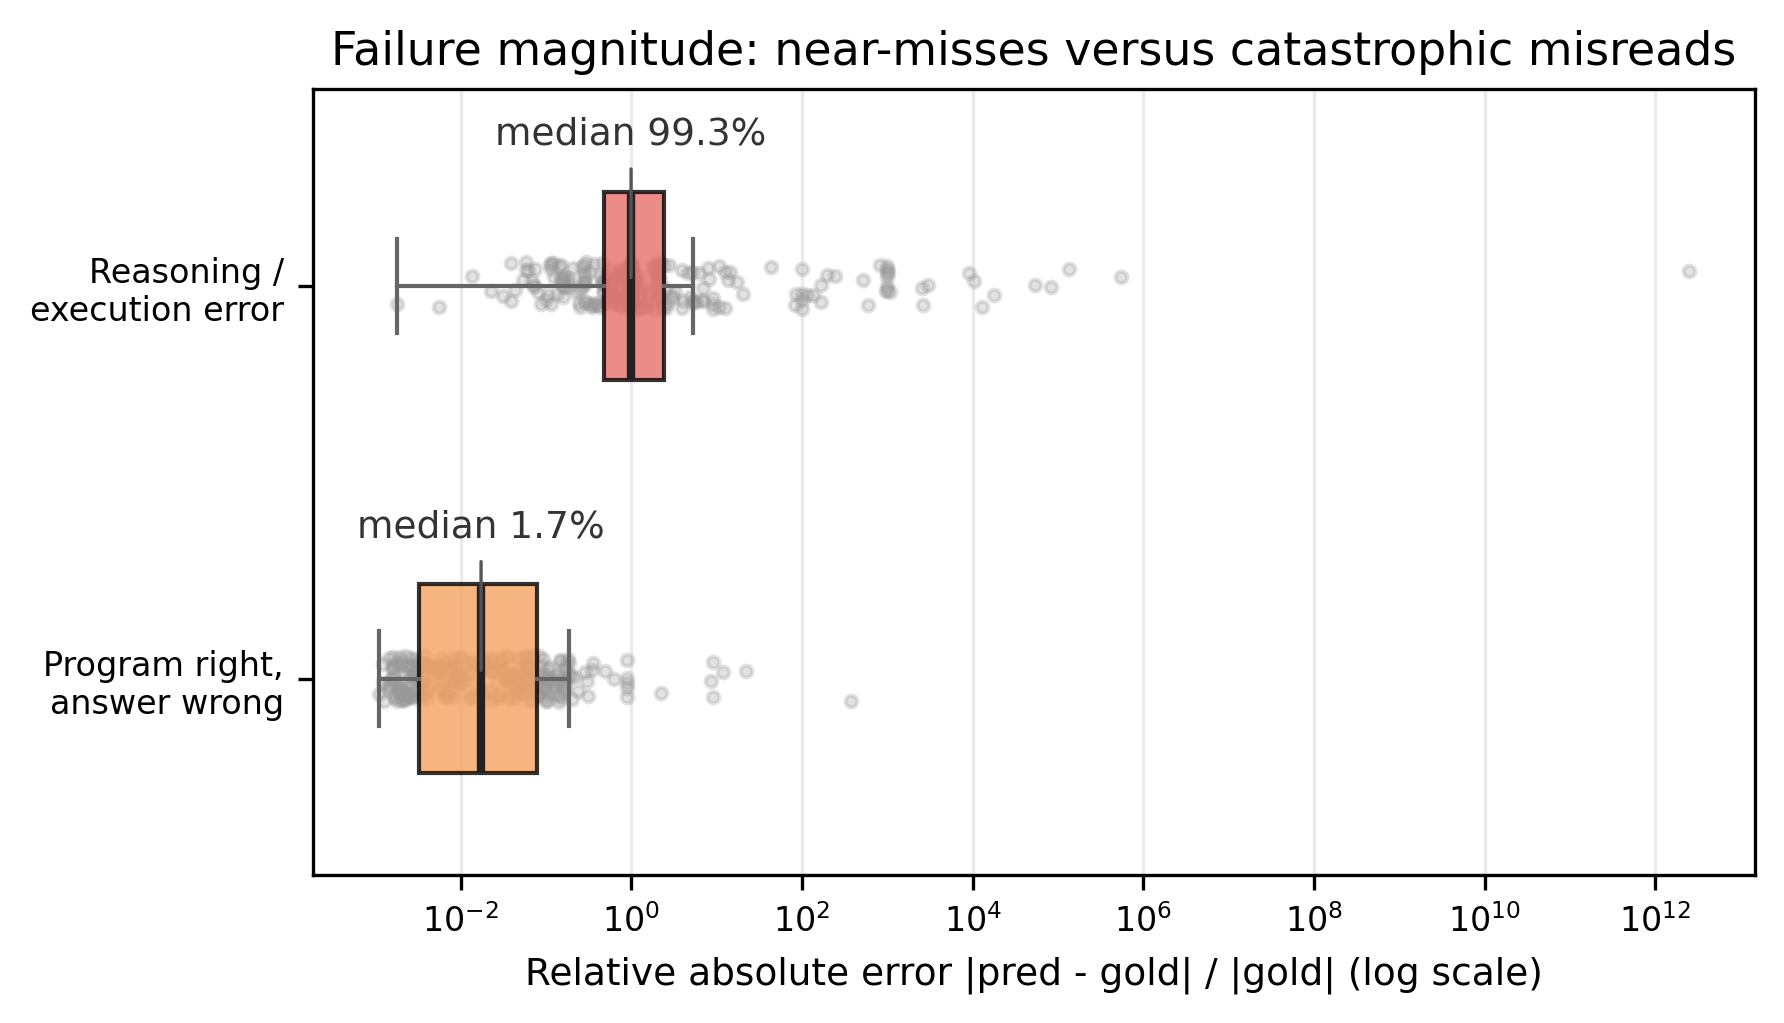
\includegraphics[width=\linewidth]{fig5_finqa_error_magnitude.png}
\caption{E5 validation absolute-error distribution for FiQA sentiment regression.}
\label{fig:fiqa-errors}
\end{figure}

\subsection{Reproducibility and resource accounting}
Each reported result is intended to be traceable through four identifiers: dataset release
and split, model and adapter checkpoint, prompt and decoding policy, and prediction export.
The Phase-3 winner uses Qwen3-1.7B with 4-bit NF4 quantization, LoRA rank 16, scaling
$\alpha=32$, dropout 0.05, learning rate $2\times10^{-4}$, weight decay 0.01, warm-up
ratio 0.03, gradient accumulation 8, two epochs, and seed 42. The Phase-4 protected run
then freezes $n=8$, temperature 0.7, top-$p$ 0.9, five-fold out-of-fold calibration, and
coverage targets 0.80 and 0.90. This separation makes it possible to distinguish a result
that was selected on validation from one that was measured after the protected freeze.

The E5 training run processed 7\,073 examples for two epochs in 2.47 hours, used a peak
3.40 GiB of VRAM on a 6 GB RTX 4050 Laptop GPU, and reported 1.18 seconds per item for
single-example inference. EVG-CAS requires 4.8 seconds per question versus 1.3 seconds for
greedy decoding in the protected profiling setup. These measurements are hardware- and
prompt-dependent; they describe the reported setup rather than a universal serving rate.

\begin{table}[t]
\centering
\caption{Reproducibility checklist for the reported experiments.}
\label{tab:repro-check}
\small
\resizebox{\columnwidth}{!}{%
\begin{tabular}{p{0.29\columnwidth}p{0.62\columnwidth}}
\toprule
item & recorded control\\
\midrule
data & split counts, source fingerprints, normalized signatures\\
training & checkpoint, QLoRA configuration, seed, sampling policy\\
evaluation & official FinQA executor, task-specific metrics\\
selection & validation-only model and threshold selection\\
protected test & freeze manifest, protected flag, post-run hash\\
artifacts & predictions, metrics, plots, and analysis summaries\\
\bottomrule
\end{tabular}}
\end{table}

\section{Discussion and limitations}
\textbf{What we did not claim.} EVG-CAS does not raise accuracy; reporting a tie, rather
than a $p$-value-won headline, is the point of the pre-registration. \textbf{Domain limits.}
On FiQA (117 validation / 234 test records, regression), the EVG features carry no signal
and the frozen policy correctly abstains to no effect --- a second reported negative result.
\textbf{General limits.} One backbone, one seed, one evaluation harness; between-seed
variance of the agreement signal is unmeasured; $n{=}8$ is pre-declared, not tuned; the
abstention gain costs 3.7$\times$ latency for zero accuracy gain. \textbf{Threats to
validity.} The protected-test protocol rests on the frozen manifest hash being unchanged
across access (it is); any leakage would invalidate C3's transfer claim. \textbf{Ethics.}
Abstention is a refusal signal, not a guarantee; a deployed system that \emph{answers} still
carries residual error (23.8\% at coverage 0.8). No financial advice is implied.

\section{Conclusion}
For a QLoRA-adapted 1.7B financial model, execution-verified generation ties greedy decoding
on accuracy but produces a steep, monotone agreement signal that the model's own confidence
cannot see. Calibrating that signal yields a pre-registered abstention threshold that
transfers to a once-opened protected test, cutting answered-error by 31\% at 80\% coverage.
The contribution to the financial-SLM conversation is an agreement-based selective-risk
signal for a small financial model, with a validation-frozen threshold and protected-test
transfer. Artifacts, frozen manifest and the full experiment trail are public; \texttt{P4-E9}
(FinTrust per-dimension evaluation) remains incomplete pending official judge scoring and is
the declared next step.

\small
\section*{References}
\begin{thebibliography}{99}
\bibitem{chen2021finqa} Z.~Chen \emph{et al.}, ``FinQA: A Dataset of Numerical Reasoning over Financial Data,'' EMNLP, 2021.
\bibitem{chen2022convfinqa} Z.~Chen \emph{et al.}, ``ConvFinQA: Exploring the Chain of Numerical Reasoning in Conversational Finance Question Answering,'' EMNLP, 2022.
\bibitem{zhu2021tatqa} F.~Zhu \emph{et al.}, ``TAT-QA: A Question Answering Benchmark on a Hybrid of Tabular and Textual Content in Finance,'' ACL, 2021.
\bibitem{phogat2024finetuning} K.~Singh~Phogat \emph{et al.}, ``Fine-tuning Smaller Language Models for Question Answering over Financial Documents,'' Findings of EMNLP, 2024.
\bibitem{yang2023fingpt} H.~Yang, X.-Y.~Liu, C.~D.~Wang, ``FinGPT: Open-Source Financial Large Language Models,'' J. Financial Data Science (arXiv:2306.06031), 2023.
\bibitem{yang2023investlm} Y.~Yang, Y.~Tang, K.~Y.~Tam, ``InvestLM: A Large Language Model for Investment using Financial Domain Instruction Tuning,'' arXiv:2309.13064, 2023.
\bibitem{wu2023bloomberg} S.~Wu \emph{et al.}, ``BloombergGPT: A Large Language Model for Finance,'' arXiv:2303.17564, 2023.
\bibitem{huang2020finbert} A.~Huang, H.~Wang, Y.~Yang, ``FinBERT: A Pretrained Language Model for Financial Communications,'' arXiv:2006.08097, 2020.
\bibitem{shi2025kronos} Y.~Shi \emph{et al.}, ``Kronos: A Foundation Model for the Language of Financial Markets,'' arXiv:2508.02739, 2025.
\bibitem{xie2024finben} Q.~Xie \emph{et al.}, ``FinBen: A Holistic Financial Benchmark for Large Language Models,'' NeurIPS D\&B, 2024.
\bibitem{hu2025fintrust} T.~Hu \emph{et al.}, ``FinTrust: A Comprehensive Benchmark of Trustworthiness Evaluation in Finance Domain,'' EMNLP, 2025.
\bibitem{subramanian2025slms} S.~Subramanian \emph{et al.}, ``Small Language Models (SLMs) Can Still Pack a Punch: A Survey,'' arXiv:2501.05465, 2025.
\bibitem{abdin2024phi3} M.~Abdin \emph{et al.}, ``Phi-3 Technical Report,'' arXiv:2404.14219, 2024.
\bibitem{zhang2024tinyllama} P.~Zhang \emph{et al.}, ``TinyLlama: An Open-Source Small Language Model,'' arXiv:2401.02385, 2024.
\bibitem{qwen2025qwen3} Qwen Team, ``Qwen3 Technical Report,'' arXiv:2505.09388, 2025.
\bibitem{hu2022lora} E.~Hu \emph{et al.}, ``LoRA: Low-Rank Adaptation of Large Language Models,'' ICLR, 2022.
\bibitem{dettmers2023qlora} T.~Dettmers \emph{et al.}, ``QLoRA: Efficient Finetuning of Quantized LLMs,'' NeurIPS, 2023.
\bibitem{wang2023selfconsistency} X.~Wang \emph{et al.}, ``Self-Consistency Improves Chain of Thought Reasoning in Language Models,'' ICLR, 2023.
\bibitem{lightman2024verify} H.~Lightman \emph{et al.}, ``Let's Verify Step by Step,'' ICLR, 2024.
\bibitem{wang2024mathshepherd} P.~Wang \emph{et al.}, ``Math-Shepherd: Verify and Reinforce LLMs Step-by-step without Human Annotations,'' ACL, 2024.
\bibitem{chen2019execution} X.~Chen, D.~Song, Y.~Tian, ``Execution-Guided Neural Program Synthesis,'' ICLR, 2019.
\bibitem{eliyaniv2010selective} R.~El-Yaniv, Y.~Wiener, ``On the Foundations of Noise-free Selective Classification,'' JMLR 11, 2010.
\bibitem{geifman2017selective} Y.~Geifman, R.~El-Yaniv, ``Selective Classification for Deep Neural Networks,'' NeurIPS, 2017.
\bibitem{geifman2019selectivenet} Y.~Geifman, R.~El-Yaniv, ``SelectiveNet: A Deep Neural Network with an Integrated Reject Option,'' ICML, 2019.
\bibitem{guo2017calibration} C.~Guo \emph{et al.}, ``On Calibration of Modern Neural Networks,'' ICML, 2017.
\bibitem{platt1999platt} J.~C.~Platt, ``Probabilistic Outputs for Support Vector Machines and Comparisons to Regularized Likelihood Methods,'' Advances in Large Margin Classifiers, 1999.
\bibitem{zadrozny2002isotonic} B.~Zadrozny, C.~Elkan, ``Transforming Classifier Scores into Accurate Multiclass Probability Estimates,'' KDD, 2002.
\bibitem{lin2022uncertainty} S.~Lin, J.~Hilton, O.~Evans, ``Teaching Models to Express Their Uncertainty in Words,'' TMLR, 2022.
\bibitem{fritzmorgenthal2022risk} S.~Fritz-Morgenthal, B.~Hein, J.~Papenbrock, ``Financial Risk Management and Explainable, Trustworthy, Responsible AI,'' SSRN 3873768, 2022.
\bibitem{cisc2025} ``Confidence Improves Self-Consistency in LLMs,'' Findings of ACL, 2025 (https://aclanthology.org/2025.findings-acl.1030/).
\bibitem{secondguess2025} ``Second Guess: Two-Pass Answer-Stability Abstention for Small-Language-Model MCQ,'' arXiv:2605.25394, 2026.
\bibitem{sconu2025} ``SConU: Selective Conformal Uncertainty Estimation for Language Models,'' ACL, 2025.
\bibitem{lec2025} ``Linear Expectation Constraints for Selection-Conditioned Risk Control,'' arXiv:2512.01556, 2025.
\bibitem{aspire2023} ``ASPIRE: Adaptation with Self-Evaluation for Selective Prediction of LLMs,'' arXiv:2310.11689, 2023.
\bibitem{finman2025} ``David vs. Goliath: Cost-Efficient Financial QA via Cascaded Multi-Agent Reasoning,'' Findings of EMNLP, 2025 (https://aclanthology.org/2025.findings-emnlp.225/).
\bibitem{gbfr2026} ``Graph-Bounded Financial Reasoning with Safe Abstention,'' 2026.
\bibitem{finchain2025} ``FinChain: Verifiable Chain-of-Thought Reasoning in Finance,'' arXiv:2506.02515, 2025.
\end{thebibliography}

\end{document}